\documentclass[11pt]{article}

\usepackage[margin=1in]{geometry}
\usepackage{amsmath,amssymb,amsthm,mathtools}
\usepackage{graphicx}
\usepackage{microtype}
\usepackage{enumitem}
\usepackage{xcolor}
\usepackage[colorlinks=true,linkcolor=blue!55!black,citecolor=blue!55!black,urlcolor=blue!65!black]{hyperref}

\newtheorem{theorem}{Theorem}
\newtheorem{proposition}[theorem]{Proposition}
\newtheorem{remark}[theorem]{Remark}
\newtheorem{definition}[theorem]{Definition}

\newcommand{\T}{\mathbb T}
\newcommand{\C}{\mathbb C}
\newcommand{\bGamma}{\widehat{\Gamma}}
\newcommand{\HS}{\mathrm{HS}}

\title{Diagonal universality and a Hilbert--Schmidt sufficient class\\
for Problem 1.5 of arXiv:2302.12857}
\author{Candidate partial result from run \texttt{fa\_banach\_001}}
\date{19 July 2026}

\begin{document}
\maketitle

\begin{center}
\fbox{\parbox{0.91\textwidth}{
\textbf{Status: candidate partial result; human review required.}
The packet does not claim a full characterization for arbitrary bounded
operators.  It proves (i) that the natural diagonal form with arbitrary
bounded operator is already universal for all bounded sequences, and (ii)
that Hilbert--Schmidt operators give genuine correlation sequences, with a
stronger two-variable commuting-action realization.
}}
\end{center}

\section{Source and exact question}

The source is Or Shalom, \emph{An application of Grothendieck theorem to the
theory of multicorrelation sequences, multiple recurrence and partition
regularity of quadratic equations}, arXiv:2302.12857v1, submitted 24 February
2023 \cite{Shalom2023}.  The question is Problem 1.5 in Section 1.1, printed
on page 4 of the source PDF.  It refers to the right-hand side of equation (2)
from Theorem 1.2 on page 3:
\[
 \int_X T_\gamma S_{\gamma'}f\,T_\gamma g\,h\,d\mu
 =\int_\Sigma (G\xi_\gamma)(\chi)\,\xi_{\gamma'}(\chi)\,d\lambda(\chi),
 \qquad \xi_\gamma(\chi)=\chi(\gamma).
\]

\begin{figure}[ht]
  \centering
  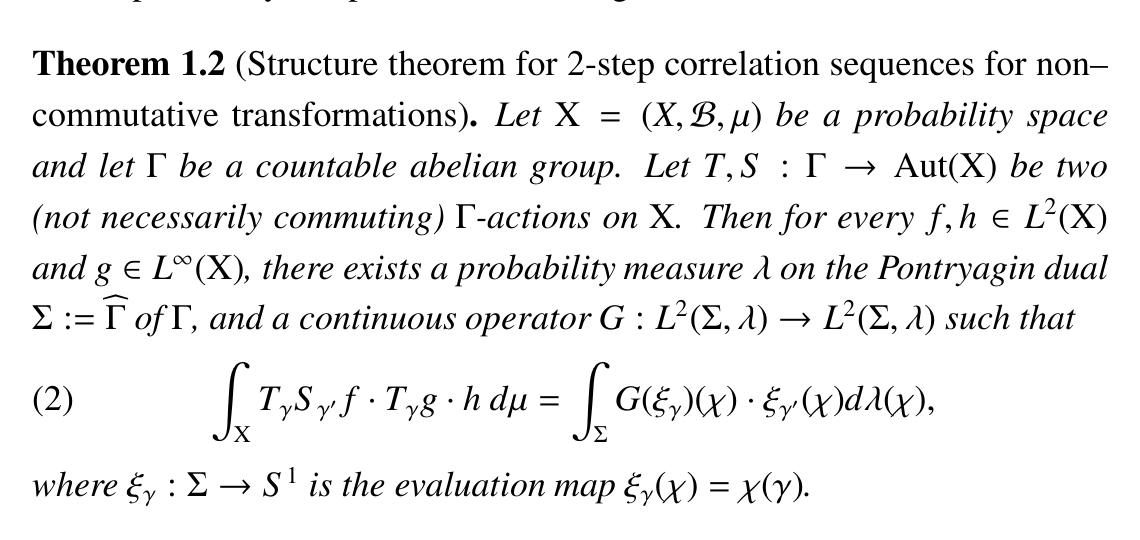
\includegraphics[width=\textwidth]{figures/source_equation_2.png}
  \caption{Equation (2) and its hypotheses, rendered from page 3 of the source PDF.}
\end{figure}

\begin{figure}[ht]
  \centering
  
\includegraphics[width=\textwidth]{figures/open_problem_crop.png}
  \caption{Problem 1.5, rendered from page 4 of the source PDF.}
\end{figure}

\paragraph{Transcription.}
``Determine for which $\lambda$ and $G$ the expression on the right hand side
of (2) is a multicorrelation sequence for commuting $T$ and $S$, or for
$T=S$.''

The displayed expression has two independent variables $\gamma,\gamma'$, but
the source definition of a multicorrelation sequence has one variable.  We
therefore separate two precise statements: a result for the full function on
$\Gamma^2$, and a result for the natural diagonal $\gamma'=\gamma$.  This
scope distinction is essential to the claims below.

\section{Definitions and conventions}

Let $\Gamma$ be a countable discrete abelian group and let
$\Sigma=\widehat\Gamma$ be its compact Pontryagin dual.  Write
$\xi_\gamma(\chi)=\chi(\gamma)$.  A $k$-step multicorrelation sequence in the
source is a function
\[
 c(\gamma)=\int_X\prod_{j=0}^{k}R_{j\gamma}f_j\,d\mu,
 \qquad f_j\in L^\infty(X),
\]
for a probability-preserving $\Gamma$-action $R$.  In particular, an ordinary
correlation $\int_X h\,R_\gamma f\,d\mu$ is a $1$-step multicorrelation and,
by adjoining factors equal to $1$, is a $k$-step multicorrelation for every
$k\geq 1$.

The source uses the bilinear pairing $\int uv\,d\lambda$, without complex
conjugation.  We use exactly this convention.  A function on $\Gamma^d$ is a
Fourier--Stieltjes transform if it has the form
\[
 \gamma\longmapsto \int_{\widehat{\Gamma^d}}\omega(\gamma)\,d\nu(\omega)
\]
for a finite complex Borel measure $\nu$.

\section{Proof Intuition}

There are two complementary mechanisms.  For Haar measure, the evaluation
characters form an orthonormal basis.  A weighted flip of this basis sends
$\xi_\gamma$ to $a(\gamma)\xi_{-\gamma}$, so the bilinear diagonal coefficient
is exactly an arbitrary prescribed bounded sequence $a(\gamma)$.  Thus mere
boundedness of $G$ cannot itself encode the desired dynamical structure.

For a Hilbert--Schmidt operator the situation changes: the operator has an
$L^2$ kernel $K(\chi,\eta)$.  Expanding the coefficient turns the entire
two-variable expression into the Fourier transform of the finite measure
$K(\chi,\eta)d\lambda(\chi)d\lambda(\eta)$ on $\Sigma^2$.  A one-circle skew
product then realizes every such Fourier transform as an ordinary correlation
of two commuting actions.  On the diagonal the two actions combine into one,
giving a multicorrelation sequence in the source's precise sense.  The
remaining open territory is the bounded non-Hilbert--Schmidt case and any
desired intrinsic characterization of those pairs $(\lambda,G)$.

\section{Candidate partial theorem}

\begin{theorem}[Universality versus the Hilbert--Schmidt class]\label{thm:main}
Let $\Gamma$ be a countable discrete abelian group,
$\Sigma=\widehat\Gamma$, and $\xi_\gamma(\chi)=\chi(\gamma)$.
\begin{enumerate}[label=\textup{(\alph*)}]
\item \textbf{Diagonal universality.}
Let $m$ be normalized Haar measure on $\Sigma$.  For every
$a\in\ell^\infty(\Gamma)$ there is a bounded linear operator
$G_a:L^2(\Sigma,m)\to L^2(\Sigma,m)$ with
\[
 \|G_a\|=\|a\|_\infty,
 \qquad
 \int_\Sigma (G_a\xi_\gamma)(\chi)\xi_\gamma(\chi)\,dm(\chi)
 =a(\gamma)
\]
for all $\gamma\in\Gamma$.  Conversely, every diagonal coefficient produced
by a probability measure $\lambda$ and a bounded $G$ is bounded, with
supremum norm at most $\|G\|$.  Hence, when arbitrary pairs $(\lambda,G)$ are
allowed, the diagonal forms are exactly $\ell^\infty(\Gamma)$.

\item \textbf{A two-variable sufficient class.}
Let $\lambda$ be any Borel probability measure on $\Sigma$ and let
$G:L^2(\Sigma,\lambda)\to L^2(\Sigma,\lambda)$ be Hilbert--Schmidt.  Then
\[
 b_G(\gamma,\gamma')
 :=\int_\Sigma (G\xi_\gamma)(\chi)\xi_{\gamma'}(\chi)\,d\lambda(\chi)
\]
is a Fourier--Stieltjes transform on $\Gamma^2$.  More strongly, there are a
probability space $(Y,\mu)$, two commuting probability-preserving
$\Gamma$-actions $T,S$, and $f,h\in L^\infty(Y)$ such that
\[
 b_G(\gamma,\gamma')
 =\int_Y T_\gamma S_{\gamma'}f\;T_\gamma 1\;h\,d\mu
 =\int_Y T_\gamma S_{\gamma'}f\;h\,d\mu.
\]

\item \textbf{Diagonal consequence.}
The diagonal $a_G(\gamma)=b_G(\gamma,\gamma)$ is an ordinary correlation
sequence for a single probability-preserving $\Gamma$-action.  It is therefore
a multicorrelation sequence under the source definition.  If $K$ is the
$L^2$ kernel of $G$, the representing Fourier--Stieltjes measure can be chosen
with total variation at most
\[
 \|K\|_{L^1(\lambda\otimes\lambda)}
 \leq \|K\|_{L^2(\lambda\otimes\lambda)}=\|G\|_{\HS}.
\]
\end{enumerate}
\end{theorem}

\begin{proof}
\textbf{Part (a).}
By Pontryagin duality and Haar orthogonality, the characters
$\{\xi_\gamma:\gamma\in\Gamma\}$ form an orthonormal basis of
$L^2(\Sigma,m)$ \cite[Chapter 1]{Rudin1962}.  Define on this basis
\[
 G_a\xi_\gamma=a(\gamma)\xi_{-\gamma}.
\]
The map $\gamma\mapsto-\gamma$ is a permutation of $\Gamma$, so for every
finitely supported scalar family $(c_\gamma)$,
\[
 \left\|G_a\sum_\gamma c_\gamma\xi_\gamma\right\|_2^2
 =\sum_\gamma |a(\gamma)c_\gamma|^2
 \leq\|a\|_\infty^2\sum_\gamma|c_\gamma|^2.
\]
Thus $G_a$ extends to a bounded linear operator.  Testing it on basis vectors
whose weights approach the supremum gives $\|G_a\|=\|a\|_\infty$.  Finally,
\[
 \int_\Sigma(G_a\xi_\gamma)\xi_\gamma\,dm
 =a(\gamma)\int_\Sigma\xi_{-\gamma}\xi_\gamma\,dm
 =a(\gamma).
\]
In the other direction, because $|\xi_\gamma|=1$ and $\lambda$ is a
probability measure, Cauchy--Schwarz gives
\[
 \left|\int_\Sigma(G\xi_\gamma)\xi_\gamma\,d\lambda\right|
 \leq \|G\xi_\gamma\|_2\|\xi_\gamma\|_2\leq\|G\|.
\]
This proves the exact universality assertion.

\medskip
\noindent\textbf{Part (b): kernel and measure.}
The Hilbert--Schmidt kernel identification gives
$K\in L^2(\Sigma\times\Sigma,\lambda\otimes\lambda)$ such that
\[
 (Gu)(\chi)=\int_\Sigma K(\chi,\eta)u(\eta)\,d\lambda(\eta)
\]
for $u\in L^2(\Sigma,\lambda)$, with
$\|K\|_2=\|G\|_{\HS}$ \cite[Chapter 2]{Simon2005}.  Since $\lambda$ is a
probability measure, $K\in L^1$.  Fubini's theorem yields
\begin{align*}
 b_G(\gamma,\gamma')
 &=\iint_{\Sigma^2}K(\chi,\eta)\eta(\gamma)\chi(\gamma')
       \,d\lambda(\eta)d\lambda(\chi)\\
 &=\int_{\Sigma^2}\eta(\gamma)\chi(\gamma')\,d\nu(\eta,\chi),
\end{align*}
where
\[
 d\nu(\eta,\chi)=K(\chi,\eta)\,d\lambda(\eta)d\lambda(\chi).
\]
This is a Fourier--Stieltjes transform on $\Gamma^2$, and
$\|\nu\|\leq\|K\|_1\leq\|K\|_2$.

\medskip
\noindent\textbf{Part (b): commuting dynamical realization.}
Write $d\nu=q\,d\rho$, where $\rho=|\nu|$, $|q|=1$ $\rho$-almost everywhere,
and let $M=\rho(\Sigma^2)$.  The case $M=0$ is immediate, so assume $M>0$.
On
\[
 Y=\Sigma\times\Sigma\times\T,
 \qquad
 \mu=\frac{\rho}{M}\otimes m_{\T},
\]
define point transformations
\[
 \tau_\gamma(\eta,\chi,z)=(\eta,\chi,\eta(\gamma)z),
 \qquad
 \sigma_{\gamma'}(\eta,\chi,z)=(\eta,\chi,\chi(\gamma')z).
\]
They are commuting probability-preserving $\Gamma$-actions: they fix the base
and rotate the Haar circle in the fibre.  Let their Koopman operators be
$T_\gamma F=F\circ\tau_\gamma$ and
$S_{\gamma'}F=F\circ\sigma_{\gamma'}$.  Put
\[
 f(\eta,\chi,z)=z,
 \qquad h(\eta,\chi,z)=M q(\eta,\chi)\overline z.
\]
Both functions are bounded.  Direct substitution gives
\begin{align*}
 \int_Y T_\gamma S_{\gamma'}f\,h\,d\mu
 &=\int_{\Sigma^2\times\T}
     \eta(\gamma)\chi(\gamma')z\,M q(\eta,\chi)\overline z
     \,d(\rho/M)\,dm_\T\\
 &=\int_{\Sigma^2}\eta(\gamma)\chi(\gamma')\,d\nu(\eta,\chi)
 =b_G(\gamma,\gamma').
\end{align*}
Taking the middle function in the source's equation (2) to be $1$ supplies
the claimed full two-variable realization.

\medskip
\noindent\textbf{Part (c).}
Because $T$ and $S$ commute, $R_\gamma=T_\gamma S_\gamma$ is a
probability-preserving $\Gamma$-action.  Consequently
\[
 a_G(\gamma)=b_G(\gamma,\gamma)=\int_Y R_\gamma f\,h\,d\mu
\]
is an ordinary correlation.  It matches the source definition with
$f_0=h$, $f_1=f$ and, for any desired larger step, all remaining functions
equal to $1$.  Equivalently, its Fourier--Stieltjes measure is the pushforward
of $\nu$ by $(\eta,\chi)\mapsto\eta\chi$.  The norm estimate was established
above.
\end{proof}

\section{Consequences and precise limitations}

\begin{enumerate}[leftmargin=*]
\item Every finite-rank, trace-class, or Hilbert--Schmidt $G$ is covered by
Theorem~\ref{thm:main}(b).  In particular, if $L^2(\Sigma,\lambda)$ is finite
dimensional, every bounded $G$ is covered.
\item Part (a) is a sharp obstruction to a characterization based only on
operator norm or generic boundedness: with the admissible Haar measure, the
diagonal construction produces every bounded sequence.
\item The theorem does \emph{not} characterize which arbitrary bounded,
non-Hilbert--Schmidt operators give multicorrelation sequences.  Nor does it
resolve whether a particular bounded sequence is a multicorrelation sequence;
the source itself identifies that classification as a major open problem.
\item The phrase ``for commuting $T$ and $S$'' in Problem 1.5 may intend a
specific one-variable specialization other than the diagonal.  The packet's
full $\Gamma^2$ realization is unambiguous and stronger at the level of the
displayed two-variable coefficient; its formal multicorrelation conclusion is
stated only for the diagonal.
\end{enumerate}

\section{Verification notes}

The accompanying \texttt{verification.md} contains an explicit adversarial
verifier report.  The main checks are:
\begin{enumerate}[leftmargin=*]
\item the weighted Fourier-basis flip is complex-linear and remains valid for
groups with $2$-torsion;
\item the source's bilinear (not sesquilinear) pairing is used throughout;
\item the order of the kernel variables gives exactly
$\eta(\gamma)\chi(\gamma')$;
\item the skew-product transformations satisfy the group laws, commute, and
preserve the probability measure;
\item the polar-density factor $M$ is placed in $h$, so the correlation has
the correct normalization and both observables are bounded;
\item setting the source's middle observable to $1$ reproduces equation (2),
and combining the commuting actions proves the diagonal claim.
\end{enumerate}
No numerical experiment is used as proof.  The only code in the packet renders
the two source crops from the copied source PDF.

\section{Bounded novelty check and review recommendation}

On 19 July 2026, the run's solution, attempt, proof-gap, and ledger indexes
were searched for arXiv:2302.12857 and for the core phrases
``Grothendieck multicorrelation'', ``for which lambda and G'',
``Hilbert--Schmidt'', and ``Fourier--Stieltjes''; no duplicate result packet
was found.  Exact-title and exact-problem web searches, the arXiv record, an
author follow-up search, and a bounded OpenAlex citation query did not locate
a later paper explicitly answering Problem 1.5.  Semantic Scholar rate-limited
the query.  A recent author paper, arXiv:2607.13286, concerns a different
non-vanishing question.  These checks are bounded and do not establish
originality.

\paragraph{Human-review recommendation.}
Treat this as a likely valid, substantial partial result.  The highest-value
review points are (i) the intended one-variable reading of Problem 1.5,
(ii) the Hilbert--Schmidt kernel convention for the source's bilinear pairing,
and (iii) whether an equivalent sufficient class or the diagonal-universality
observation already appears under different terminology.  Do not promote it
to a full solution without a characterization of the arbitrary bounded case.

\begin{thebibliography}{9}
\bibitem{Shalom2023}
O. Shalom,
\emph{An application of Grothendieck theorem to the theory of multicorrelation
sequences, multiple recurrence and partition regularity of quadratic
equations}, arXiv:2302.12857v1 (2023),
\url{https://arxiv.org/abs/2302.12857}.

\bibitem{Rudin1962}
W. Rudin,
\emph{Fourier Analysis on Groups},
Interscience Publishers, 1962.

\bibitem{Simon2005}
B. Simon,
\emph{Trace Ideals and Their Applications}, 2nd ed.,
American Mathematical Society, 2005.
\end{thebibliography}

\end{document}
